\section{Image Retrieval}
	\indent    In week 4, we got familiar with the instance retrieval process. We worked on a subset of the ImageNet dataset containing of 2 classes (dog and car). For each class were used 5000 images for training and 150 images for testing. We tested different values for many parameters(detector, descriptor, num. of k-means centroids, global descriptor and query technique). We obtained best results on the following setting: dense sampling for detector, SIFT local descriptor, k=50, Fisher as global descriptor and fast nearest-neighbor for querying. Using those, we recorded top5 accuracy of \textbf{84\%}. That result is highlighted below on dedicated figure, where other results are also shown. 
\par	Using VLAD as a global descriptor, we did not get satisfactory results. With parameters set to k=200 for k-means and fast nearest neighbor querying, dense sampling for detecting features and SIFT for local describing, the top5 performance of the model maxed out at 69\%. We also tested other layouts, like FAST/SIFT and DENSE/SURF for detector/descriptor accordingly, which were less effective. From here on, we used combination of dense sampling and SIFT for local descriptor in the following tests for BoW and Fisher vector as global descriptor.

\centerline{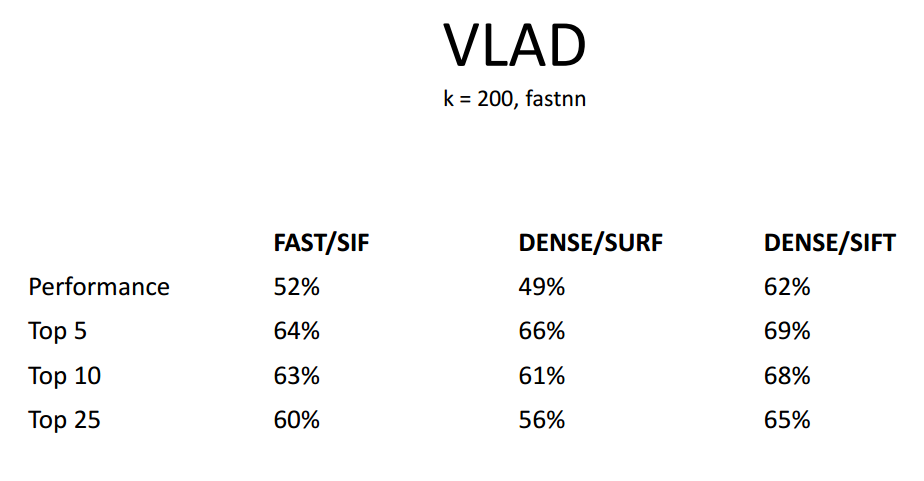
\includegraphics[scale = 0.5]{figures/vlad.png}}

\par Bag of Words as global descriptor performed admirably. We recorded the best performance with vocabulary of size k=500, dense+sift and fast n.n. querying technique, obtaining 79\% top5 accuracy.
\par	Fisher vectors proved to be the best method in our tests. As previously said, the best result we had was 84\% accuracy on top5 with fastnn query. We also tried product quantization (with the default  number of partitions) and locality sensitive hashing on PQ for querying algorithms, which proved to be comparable on smaller vocabulary sizes, but failed to deliver better results on bigger.

\centerline{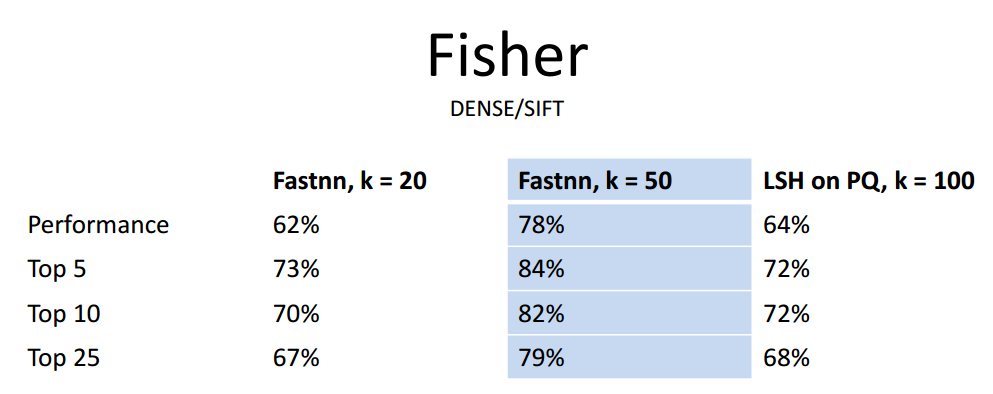
\includegraphics[scale = 0.5]{figures/fish.png}}

\par We are able to conclude that Fisher did perform the best here with vocabulary of only 50 words, but with larger vocabularies it gets too heavy dimensionality-wise as a consequence of the method. Therefore, even 50 words vocabulary with Fisher vector computes slower than 500 words vocabulary on BoW, for example. While dimensionality becomes a big problem for Fisher vectors, also for other techniques we can say that parallelization is a must, since computational cost is heavy on these tasks.
